\documentclass[letterpaper]{article}
\usepackage[T1]{fontenc}
\usepackage[utf8]{inputenc}
\usepackage[spanish,es-tabla]{babel}
\usepackage[lmargin=3cm,rmargin=3cm,top=3cm,bottom=3cm]{geometry}
\usepackage{amsmath,amsfonts}
\usepackage{mathtools}
\usepackage{graphicx}
\usepackage{fancyhdr}
\usepackage{caption}


\lhead{Universidad del Bío-Bío\\ Facultad de ingeniería \\ Escuela de Ingeniería Industrial}
\rhead{\begin{picture}(0,0) \put(-75,0){
\includegraphics[height=15mm]{logos/escudo_ubb_2}} \end{picture}}

\pagestyle{fancy}


\usepackage{titlesec}
\titleformat*{\section}{\large\bfseries\centering}
\titleformat*{\subsection}{\normalsize\bfseries}

\begin{document}
\vspace*{0.1\baselineskip}
\section*{Práctica 5}
\subsection*{Problema 1}
Dado un grafo $G=(N,A)$ con $N$ el conjunto de nodos clientes y $A$ el conjunto de arcos, $c_{ij}$ el costo y $d_{ij}$ la distancia del arco $(i,j)$. El problema consiste en localizar un path que comienza en un nodo origen $s$ y termina en un nodo destino $t$. Ambos nodos extremos del path son dados a priori, con $s,t \in N$. Todos los clientes que no están en el path deben ser asignados al nodo más cercano que se encuentre en el mismo path. Se quiere minimizar el costo del path y la distancia total que recorre cada uno de los clientes para alcanzar el nodo sobre el path que le es asignado.
\begin{itemize}
\item Construya una pequeña red para mostrar una solución factible del problema, esto es, indicar los nodos extremos, el path y mediante arcos la asignación de los clientes al path
\item Establezca los supuestos que estime conveniente, describa los parámetros y defina las variables de decisión
\item Formule un modelo de programación lineal entera que permita resolver este problema
\end{itemize}

\subsection*{Problema 2}
Para promover la seguridad en el campus el Departamento de Seguridad Pública de la Universidad de Arkansas se encuentra en proceso de instalación de teléfonos de emergencia en lugares seleccionados. El departamento desea instalar una cantidad mínima de estos aparatos que presten servicio
a cada una las calles principales del campus. La figura \ref{fig_1} es un mapa de dichas calles.

\begin{figure}[ht]
\centering
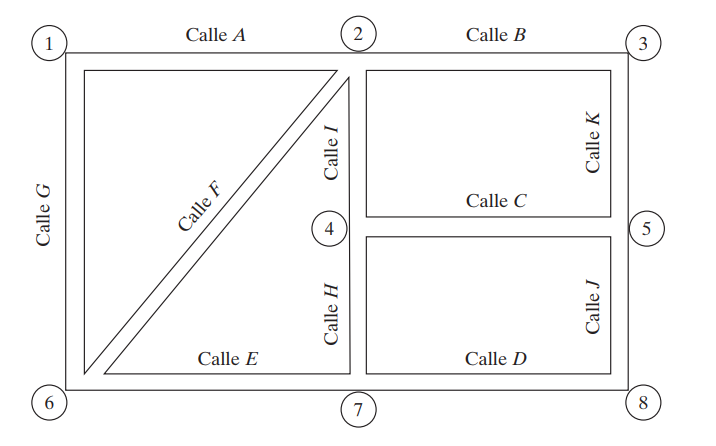
\includegraphics[width=0.7\textwidth]{images/img_1.png}
\caption{Mapa de las calles del campus de la Universidad de Arkansas}
\label{fig_1}
\end{figure}
\begin{itemize}
\item Formule un modelo de programación lineal entera que permita minimizar el número total de teléfonos, considerando que cada calle debe tener a lo menos uno.
\end{itemize}
\end{document}
